\documentclass[a4paper, 12pt]{article}

%•	Lucrarea se recomandă a avea între 30 și 60 de pagini
%•	Format: A4, fonturi de 12pt, distanță de 1.5 între rânduri
%•	Obligatoriu paginile sunt numerotate
%•	Capitolele vor începe pe pagină nouă
% margini: top=2.5cm,left=3cm,right=2.5cm,bottom=2.5cm
\usepackage{comment}
\usepackage{setspace}

% for bibliography
\usepackage[english]{babel}
\usepackage[nottoc]{tocbibind}
% for clicking on a cite leading to bibliography
\usepackage{hyperref}
\hypersetup{
    colorlinks=true,
    linkcolor=black,
    citecolor=blue,
    urlcolor=blue,
    filecolor=blue, 
}
% specificatii in legatura cu margini
\usepackage[top=2.5cm,left=3cm,right=2.5cm,bottom=2.5cm]{geometry}

\usepackage{graphicx}

% Redefine \maketitle to customize title layout
\makeatletter
\renewcommand{\maketitle}{
    \begin{center}
            \normalsize{BABEŞ-BOLYAI UNIVERSITY CLUJ-NAPOCA}\par % University name
            \normalsize{FACULTY OF MATHEMATICS AND COMPUTER SCIENCE}\par % Faculty name
            \normalsize{COMPUTER SCIENCE IN ROMANIAN SPECIALIZATION}\par
        \vspace{21em} % Vertical space

        {\LARGE\@title\par} % Title in large font
        \vspace{21em} % Vertical space

        \textbf{Supervisor}\hspace{20em}\textbf{Author}\par
        Prof.dr. Horia F. Pop\hspace{16em}{\large\@author\par} % Author
        \vspace{3em} % Vertical space

        {\large\@date\par} % Date
    \end{center}
}
\makeatother

\title{
    DIPLOMA THESIS \\
    Alzheimer's Disease Detection
}
\author{Ichim Ștefan}
\date{2024}

% Set line spacing to 1.5
\onehalfspacing

\begin{document}

% title page
\maketitle
\newpage

% ------------------------------------ABSTRACT--------------------------------------
% abstract page
\begin{abstract}
    Lorem ipsum Lorem ipsum Lorem ipsum Lorem ipsum
    Lorem ipsum Lorem ipsum Lorem ipsum Lorem ipsum
    Lorem ipsum Lorem ipsum Lorem ipsum Lorem ipsum
    Lorem ipsum Lorem ipsum Lorem ipsum Lorem ipsum
    Lorem ipsum Lorem ipsum Lorem ipsum Lorem ipsum
    Lorem ipsum Lorem ipsum Lorem ipsum Lorem ipsum
    Lorem ipsum Lorem ipsum Lorem ipsum Lorem ipsum
    Lorem ipsum Lorem ipsum Lorem ipsum Lorem ipsum
\end{abstract}
\newpage

% ------------------------------------CONTENTS--------------------------------------
\tableofcontents
\newpage

% ----------------------------------INTRODUCTION------------------------------------
\section{Introduction}
There is no denying that humanity stands at a previously inconceivable point in healthcare and medicine,
which naturally have led to hindrances in senescence, populations increasingly reaching older stages of life.
Furthermore, studies which take into account multiple case scenarios show that population is expected to reach
9.2 billion by the age of 2050, leading to an uprise of 21\% in the elderly. \cite{KC2017181}

With that being said, researchers' concern has has taken a turn towards diseases occurring at these later
parts of human lives, some of them considered treatable while others less so.
One of such disorders is Alzheimer's Disease, or AD, considered to be the most likely predecessor of dementia.
Alzheimer's Disease is a brain disease, neurodegenerative, which in time diminishes cognitive skills such as memory,
thinking and speaking, and in due course even removes the ability of accomplishing simple activities vital to one's
daily life.
On top of that, it is an incurable disorder, which only underlines even further the reasons why early
detection stand of such great importance, so that appropriate actions can be taken by both the medical team
and the one diagnosed, along with their relatives and close ones.

The brain of a healthy human represents a cluster of neurons by the number of bilions which together amount to
what actions and reactions we have, through a process of signal propagating.
Through our sensory mechanism, which includes hearing and seeing, receptors carry out the tasks of sending signals
(Fig \ref{fig:neuron-communication}) using designated channels all the way to the neurons inside the brain, where new
specific signals are formed and sent back, resulting in what we call actions. \cite{Sivadas2020HowDM}

\begin{figure}[htbp]
    \centering
    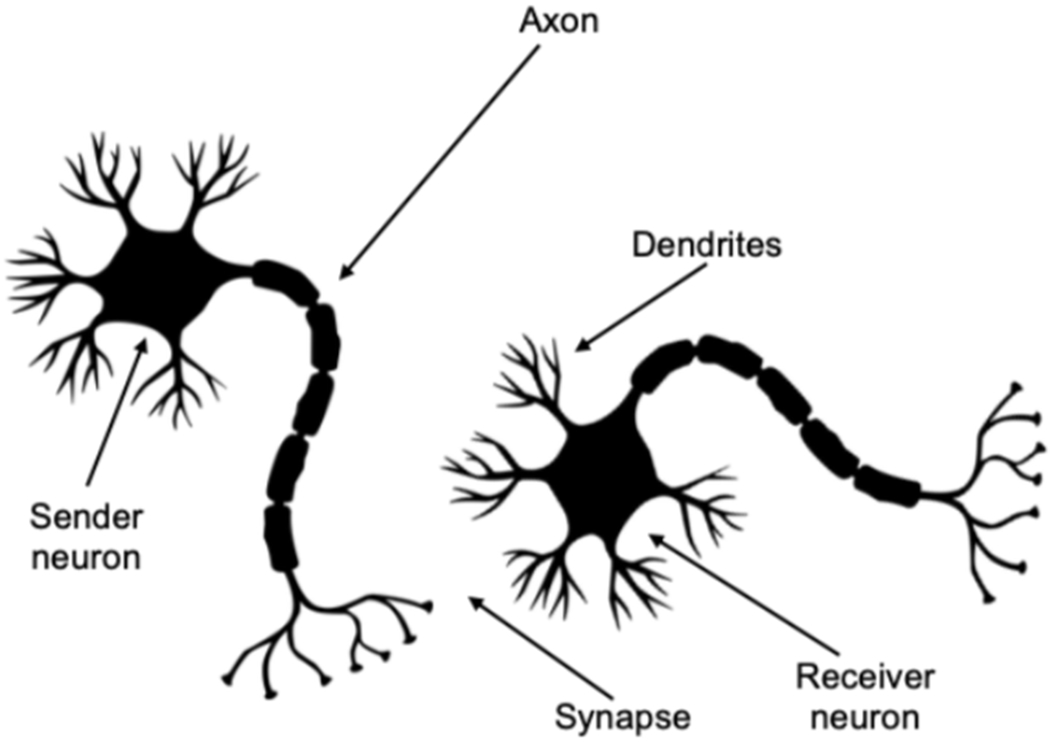
\includegraphics[width=0.65\textwidth]{figs/neuron-communication.jpg} % Change 'example-image' to the filename of your image
    \caption{Communication between neurons} % Caption for the figure
    \label{fig:neuron-communication} % Label to refer to the figure in the text
\end{figure}

Alzheimer's Disease intervenes in this process by gradually decreasing the utility function of each neuron, leading to
the atrophy of the brain's proficiencies, as neurons imminently die one by one.

There are three major factors included in the dynamic between AD and neurons.
First of all, a key advantage of neurons which many other cells lack, and which accomplishes
their long survival, is the ability to repair themselves, form new connections, or changing current ones' magnitude.
Secondly, synaptic connections, which solidify the signal transmission process, and lastly the intake of glucose and
oxygen necessary for their normal functioning.
It is believed these fundamental attributes of a healthy human receive considerable drawbacks upon the disease's presence.
\cite{NIH1}

\subsection*{Causes} % -- Introduction/Causes
While the factors which lead to Alzheimer's Disease are not yet properly understood, past research and studies prove that some
of the most commonly met criterias which lead to a diagnostic include genetic inheritance - chances of developing Alzheimer's
Disease increase by 30\% when another close relative suffers from it \cite{HMS20192801}, lifestyle and environmental factors.

\subsubsection*{Genetical Inheritance} % -- Introduction/Causes/GeneticalInheritance
Genes represent instructions passed down from generation to generation, which contain information regarding how various cells
need to behave. Some roles played by these include defining one's height, or the color of hair and eyes.

Advances in genetic research have led to discover 80 genetic areas that can possibly play a part in AD development \cite{NIH2}.
One of the more known genes which raises the risk of Alzheimer's Disease is the apolipoprotein E (APOE) gene, which comes in forms such as
$\epsilon_2, \epsilon_3, \epsilon_4$. A pair of two such APOE genes, one from each parent, gets passed down to the next generation
resulting in 6 possible cases. Among them, the $\left(\epsilon_4,\epsilon_4\right)$ combination having the highest risk of AD,
only increasing, not guaranteeing it, and in contrast, $\epsilon_2$ provides a higher degree of protection against it.

\subsubsection*{External Factors} % -- Introduction/Causes/ExternalFactors
Besides genetical inheritance, researchers have drawn conclusions regarding causes of Alzheimer's Disease to contain a plethora
of other outside factors, which we can have a higher influence on.
Among these can be found vascular conditions - high blood pressure, heart diseases - and metabolic diseases - obesity and diabetes
\cite{NIH2}.

\subsection*{Symptoms} % -- Introduction/Symptoms
Before beginning the discussion about its effects, a noteworthy fact is that brain structure modifications, whether they may be
neurofibrillary tangles or plaques of amyloid, occur several years before any cognitive issues manifest at all, a stage of the disease titled
preclinical.

\newpage


\bibliographystyle{plainnat} % Specify bibliography style
\bibliography{references}

\end{document}
